\chapter{Programming Interface for {\MPI}}

   This chapter describes the programming interface for {\MPI},
   which are widely used for parallel programming for cluster computing.
   Users can introduce {\MPI} functions to {\XMP} using the interface.   

   {\XMP} provides the following user API functions to mix {\MPI}
   functions with {\XMP}.

\begin{itemize}
\item {\tt xmp\_get\_mpi\_comm}
\item {\tt xmp\_init\_mpi}
\item {\tt xmp\_finalize\_mpi}
\end{itemize}

\section{\tt xmp\_get\_mpi\_comm}
\index{xmp\_get\_mpi\_comm@{\tt xmp\_get\_mpi\_comm}}

\subsubsection*{Format}

\begin{tabular}{lll}
\verb![F]!&  {\tt integer function}& {\tt xmp\_get\_mpi\_comm()}\\
\verb![C]!&  {\tt MPI\_Comm}& {\tt xmp\_get\_mpi\_comm(void)}
\end{tabular}

\subsubsection*{Synopsis}

   {\tt xmp\_get\_mpi\_comm} returns the handle of the communicator
   associated with the executing node set. 

\subsubsection*{Arguments}

none.

\section{\tt xmp\_init\_mpi}
\index{xmp\_init\_mpi@{\tt xmp\_init\_mpi}}

\subsubsection*{Format}

\begin{tabular}{lll}
\verb![F]!&  {\tt }& {\tt xmp\_init\_mpi()}\\

\verb![C]!&  {\tt void}& {\tt xmp\_init\_mpi(int *args, char ***argv)}
\end{tabular}

\subsubsection*{Synopsis}

   {\tt xmp\_init\_mpi} initializes the MPI execution environment.

\subsubsection*{Arguments}

   In {\XMPC}, the command-line arguments {\tt argc} and {\tt argv}
   should be given to {\tt xmp\_init\_mpi}.


\section{\tt xmp\_finalzie\_mpi}
\index{xmp\_finalzie\_mpi@{\tt xmp\_finalzie\_mpi}}

\subsubsection*{Format}

\begin{tabular}{lll}
\verb![F]!&  {\tt }& {\tt xmp\_finalize\_mpi()}\\

\verb![C]!&  {\tt void}& {\tt xmp\_finalize\_mpi(void)}
\end{tabular}

\subsubsection*{Synopsis}

   {\tt xmp\_finalize\_mpi} terminates the MPI execution enviroment.

\subsubsection*{Arguments}

   none.

\section*{Example}
\index{Example!MPI interface}

\begin{XCexample}
#include <stdio.h>
#include "mpi.h"
#include "xmp.h"

#pragma xmp nodes p(4)

int main(int argc, char *argv[]) {
  xmp_init_mpi(&argc, &argv)

  int rank, size;
  MPI_Comm_rank(MPI_COMM_WORLD, &rank);
  MPI_Comm_size(MPI_COMM_WORLD, &size);

#pragma xmp task on p(2:3)
{
  MPI_Comm comm = xmp_get_mpi_comm(); // get the MPI communicator of p(2:3)

  int rank, size;
  MPI_Comm_rank(comm, &rank);
  MPI_Comm_size(comm, &size);
}

  xmp_finalize_mpi();

  return 0;
}
\end{XCexample}

\cleardoublepage

\chapter{Directive for Thread Parallelism}
\index{Directive!threads clause@{\tt threads} clause}

Thread-level parallelism is needed to program multi-core cluster system.
Users can use some features introduced from {\OMP} to parallelize loops
in thread level with the {\tt threads} clause of the {\tt loop}
directive. No direct use of {\OMP} directives in {\XMP} code is
allowed.

\section{{\tt threads} clause}
\index{threads clause@{\tt threads} clause}

\subsection*{Syntax}
\Syntax{loop}

\begin{tabular}{ll}
\verb![F]! & \verb|!$xmp| {\tt loop} {\openb} \verb|(| {\it loop-index}
 {\openb}, {\it loop-index}{\closeb}... \verb|)| {\closeb} \\
 & \hspace{3cm}{\tt on} \{{\it nodes-ref} $\vert$ {\it template-ref}\}
     {\openb} {\it reduction-clause} {\closeb}...
     {\openb} {\it threads-clause} {\closeb} \\
 & {\it do-loops} \\
 & \\
\verb![C]! & \verb|#pragma xmp| {\tt loop} {\openb} \verb|(| {\it
     loop-index} {\openb}, {\it loop-index}{\closeb}... \verb|)|
     {\closeb} \\
 & \hspace{3cm}{\tt on} \{{\it nodes-ref} $\vert$ {\it template-ref}\}
     {\openb} {\it reduction-clause} {\closeb}...
     {\openb} {\it threads-clause} {\closeb} \\
 & {\it for-loops} \\
\end{tabular}

\vspace{0.3cm}

where {\it threads-clause} is:

\vspace{0.3cm}

\begin{tabular}{ll}
 & {\tt threads} {\openb} {\it omp-clause} {\closeb} \\
\end{tabular}

\vspace{0.3cm}

and {\it omp-clause} is one of:

\vspace{0.3cm}

\begin{tabular}{ll}
 & {\tt num\_threads(} {\it num-thread} {\tt )}\\
 & {\tt private(} {\it list} {\tt )}\\
 & {\tt firstprivate(} {\it list} {\tt )}\\
 & {\tt lastprivate(} {\it list} {\tt )}\\
\end{tabular}

\subsection*{Description}

   {\OMP} clauses such as {\tt num\_threads} can be specified in {\tt
   threads} clause.
   The {\XMP} compiler generates internally {\OMP} directives from the
   {\tt loop} directive and the {\tt threads} clause.
   Note that no {\tt reduction} need to be specified in the {\tt
   threads} clause because it is inherited from the {\tt reduction}
   clause in the {\tt loop} directive.

\subsection*{Example}
\index{Example!OpenMP interface}

   This example calculates the total sum of an array.
   A {\tt threads} clause is given to the {\tt loop} directive to
   parallelize the loop statement in both process and
   thread level. 
   The {\tt reduction} clause in the {\tt loop} directive is also
   applied to the {\OMP} directive which is generated by the {\XMP}
   compiler.

\begin{XCexample}
#include <stdio.h>
#include "xmp.h"
#define N 1024

#pragma xmp nodes p(*)
#pragma xmp template t(0:N-1)
#pragma xmp distribute t(block) onto p
#pragma xmp align a[i] with t(i)

int main(void) {
  . . . // initialize a[]

  int sum = 0;
#pragma xmp loop on t(i) reduction(+:sum) threads num_threads(4)
  for (int i = 0; i < N; i++) {
    sum += a[i];
  }

  return 0;
}
\end{XCexample}

\cleardoublepage

\chapter{Interface to Numerical Libraries}
\label{chap:Interface to Numerical Libraries}
\index{library interface}

   This chapter describes the XcalableMP interfaces to existing MPI
   parallel libraries, which is effective to achieve high productivity
   and performance of {\XMP} programs.
   
\section{Design of the Interface}

A recommended design of the interface is as follows:

\begin{itemize}

 \item Numerical library routines can be invoked by an {\XMP} procedure
       through an interface procedure (Figure \ref{figb.1}).

 \begin{myfigure}
  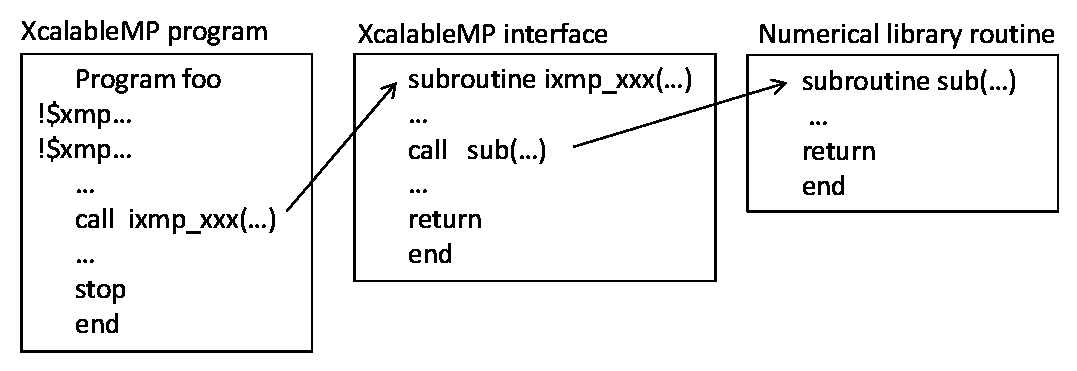
\includegraphics[scale=0.45]{figs/figb.1.eps}
  \caption{Invocation of a Library Routine through an Interface Procedure}
  \label{figb.1}
 \end{myfigure}

 \item When the numerical library routine needs information on an global
       array, the interface extracts it from the descriptor using some
       query routines provided by {\XMP} and passes it to the
       numerical library routine as arguments.
%
 \item The interface does not affect the behavior of numerical library
       routines except for restrictions concerning the {\XMP}
       specification.
\end{itemize}


\section{Query routines}

Specifications of some query routines are shown below.

\subsection{\tt xmp\_node\_index}
\index{xmp\_node\_index@{\tt xmp\_node\_index}}

\subsubsection*{Format}

\begin{tabular}{lll}

\verb![F]!& {\tt subroutine}& {\tt xmp\_node\_index(d, idx)}\\
          & {\tt integer(kind=xmp\_desc\_kind)} & {\tt d}\\
          & {\tt integer} & {\tt idx(dim)}\\

\verb![C]!&  {\tt void}& {\tt xmp\_node\_index(xmp\_desc\_t d, int idx[])}\\

\end{tabular}

\subsubsection*{Synopsis}

The {\tt xmp\_node\_index} routine provides the indices of the
executing node in the target node array.

\subsubsection*{Arguments}

\begin{itemize}
 \item {\tt d} is a descriptor, that is, an object of type {\tt
       integer(kind=xmp\_desc\_kind)}, in {\XMP}, or {\tt xmp\_desc\_t},
       in {\XMPC}, that is associated with the node array.
 \item {\tt idx} is a one-dimensional integer array. {\tt
       dim} is the rank of the node array.
\end{itemize}


\subsection{\tt xmp\_node\_size}
\index{xmp\_node\_size@{\tt xmp\_node\_size}}

\subsubsection*{Format}

\begin{tabular}{lll}

\verb![F]!& {\tt subroutine}& {\tt xmp\_node\_size(d, size)}\\
          & {\tt integer(kind=xmp\_desc\_kind)} & {\tt d}\\
          & {\tt integer} & {\tt size(dim)}\\

\verb![C]!&  {\tt void}& {\tt xmp\_node\_size(xmp\_desc\_t d, int size[])}\\

\end{tabular}

\subsubsection*{Synopsis}

The {\tt xmp\_node\_size} routine provides the size of each dimension of
the target node array.

\subsubsection*{Arguments}

\begin{itemize}
 \item {\tt d} is a descriptor, that is, an object of type {\tt
       integer(kind=xmp\_desc\_kind)}, in {\XMP}, or {\tt xmp\_desc\_t},
       in {\XMPC}, that is associated with the node array.
 \item {\tt size} is a one-dimensional integer array. {\tt
       dim} is the rank of the node array.
\end{itemize}

\subsection{\tt xmp\_gt\_size}
\index{xmp\_gt\_size@{\tt xmp\_gt\_size}}

\subsubsection*{Format}

\begin{tabular}{lll}

\verb![F]!& {\tt subroutine}& {\tt xmp\_gt\_size(d, size)}\\
          & {\tt integer(kind=xmp\_desc\_kind)} & {\tt d}\\
          & {\tt integer} & {\tt size(dim)}\\

\verb![C]!&  {\tt void}& {\tt xmp\_gt\_size(xmp\_desc\_t d, int size[])}\\

\end{tabular}

\subsubsection*{Synopsis}

The {\tt xmp\_gt\_size} routine provides the global size of each
dimension of the target template.

\subsubsection*{Arguments}

\begin{itemize}
 \item {\tt d} is a descriptor, that is, an object of type {\tt
       integer(kind=xmp\_desc\_kind)}, in {\XMP}, or {\tt xmp\_desc\_t},
       in {\XMPC}, that is associated with the target template.
 \item {\tt size} is a one-dimensional integer array. {\tt
       dim} is the rank of the template.
\end{itemize}

\subsection{\tt xmp\_lt\_size}
\index{xmp\_lt\_size@{\tt xmp\_lt\_size}}

\subsubsection*{Format}

\begin{tabular}{lll}

\verb![F]!& {\tt subroutine}& {\tt xmp\_lt\_size(d, size)}\\
          & {\tt integer(kind=xmp\_desc\_kind)} & {\tt d}\\
          & {\tt integer} & {\tt size(dim)}\\

\verb![C]!&  {\tt void}& {\tt xmp\_lt\_size(xmp\_desc\_t d, int size[])}\\

\end{tabular}

\subsubsection*{Synopsis}

The {\tt xmp\_lt\_size} routine provides the local size of each dimension
of the target template.

\subsubsection*{Arguments}

\begin{itemize}
 \item {\tt d} is a descriptor, that is, an object of type {\tt
       integer(kind=xmp\_desc\_kind)}, in {\XMP}, or {\tt xmp\_desc\_t},
       in {\XMPC}, that is associated with the template.
 \item {\tt size} is a one-dimensional integer array. {\tt
       dim} is the rank of the template.
\end{itemize}


\subsection{\tt xmp\_ga\_size}
\index{xmp\_ga\_size@{\tt xmp\_ga\_size}}

\subsubsection*{Format}

\begin{tabular}{lll}

\verb![F]!& {\tt subroutine}& {\tt xmp\_ga\_size(d, size)}\\
          & {\tt integer(kind=xmp\_desc\_kind)} & {\tt d}\\
          & {\tt integer} & {\tt size(dim)}\\

\verb![C]!&  {\tt void}& {\tt xmp\_ga\_size(xmp\_desc\_t d, int size[])}\\

\end{tabular}

\subsubsection*{Synopsis}

The {\tt xmp\_ga\_size} routine provides the global size of each
dimension of the target global array.

\subsubsection*{Arguments}

\begin{itemize}
 \item {\tt d} is a descriptor, that is, an object of type {\tt
       integer(kind=xmp\_desc\_kind)}, in {\XMP}, or {\tt xmp\_desc\_t},
       in {\XMPC}, that is associated with the global array.
 \item {\tt size} is to be set to a one-dimensional integer array. {\tt
       dim} is the rank of the global array.
\end{itemize}

\subsection{\tt xmp\_la\_size}
\index{xmp\_la\_size@{\tt xmp\_la\_size}}

\subsubsection*{Format}

\begin{tabular}{lll}

\verb![F]!& {\tt subroutine}& {\tt xmp\_la\_size(d, size)}\\
          & {\tt integer(kind=xmp\_desc\_kind)} & {\tt d}\\
          & {\tt integer} & {\tt size(dim)}\\

\verb![C]!&  {\tt void}& {\tt xmp\_la\_size(xmp\_desc\_t d, int size[])}\\

\end{tabular}

\subsubsection*{Synopsis}

The {\tt xmp\_la\_size} routine provides the local size of each
dimension of the global array.

\subsubsection*{Arguments}

\begin{itemize}
 \item {\tt d} is a descriptor, that is, an object of type {\tt
       integer(kind=xmp\_desc\_kind)}, in {\XMP}, or {\tt xmp\_desc\_t},
       in {\XMPC}, that is associated with the global array.
 \item {\tt size} is a one-dimensional integer array. {\tt
       dim} is the rank of the global array.
\end{itemize}

\subsection{\tt xmp\_ga\_template\_unitsize}
\index{xmp\_ga\_template\_unitsize@{\tt xmp\_ga\_template\_unitsize}}

\subsubsection*{Format}

\begin{tabular}{lll}

\verb![F]!&  {\tt subroutine}& {\tt xmp\_ga\_template\_unitsize(d, unitsize)}\\
          & {\tt integer(kind=xmp\_desc\_kind)} & {\tt d}\\
          & {\tt integer} & {\tt unitsize(dim)}\\

\verb![C]!&  {\tt void}& {\tt xmp\_ga\_template\_unitsize(xmp\_desc\_t d, int unitsize[])}\\

\end{tabular}

\subsubsection*{Synopsis}

The {\tt xmp\_ga\_template\_unitsize} routine provides the blocking
factor of each dimension of the target template.

\subsubsection*{Arguments}

\begin{itemize}
 \item {\tt d} is a descriptor, that is, an object of type {\tt
       integer(kind=xmp\_desc\_kind)}, in {\XMP}, or {\tt xmp\_desc\_t},
       in {\XMPC}, that is associated with the template.
 \item {\tt unitsize} is a one-dimensional integer array. {\tt dim} is
       the rank of the template.
\end{itemize}


\subsection{\tt xmp\_ga\_first\_idx\_node\_index}
\index{xmp\_ga\_first\_idx\_node\_index@{\tt
xmp\_ga\_first\_idx\_node\_index}}

\subsubsection*{Format}

\begin{tabular}{lll}

\verb![F]!&  {\tt subroutine}& {\tt xmp\_ga\_first\_idx\_node\_index(d, idx)}\\
          & {\tt integer(kind=xmp\_desc\_kind)} & {\tt d}\\
          & {\tt integer} & {\tt idx(dim)}\\

\verb![C]!&  {\tt void}& {\tt xmp\_ga\_first\_idx\_node\_index(xmp\_desc\_t d, int idx[])}\\

\end{tabular}

\subsubsection*{Synopsis}

The {\tt xmp\_ga\_first\_idx\_node\_index} routine provides the indices
of the node onto which the {\it first} element of the global array is
distributed.

\subsubsection*{Arguments}

\begin{itemize}
 \item {\tt d} is a descriptor, that is, an object of type {\tt
       integer(kind=xmp\_desc\_kind)}, in {\XMP}, or {\tt xmp\_desc\_t},
       in {\XMPC}, that is associated with the global array.
 \item {\tt idx} is a one-dimensional integer array. {\tt dim} is the
       rank of node array associeted with the global array.
\end{itemize}


\subsection{\tt xmp\_la\_lead\_dim}
\index{xmp\_la\_lead\_dim@{\tt xmp\_la\_lead\_dim}}

\subsubsection*{Format}

\begin{tabular}{lll}

\verb![F]!&  {\tt subroutine}& {\tt xmp\_la\_lead\_dim(d, lead\_dim)}\\
          & {\tt integer(kind=xmp\_desc\_kind)} & {\tt d}\\
          & {\tt integer} & {\tt lead\_dim}\\

\verb![C]!&  {\tt void}& {\tt xmp\_la\_lead\_dim(xmp\_desc\_t d, int lead\_dim)}\\

\end{tabular}

\subsubsection*{Synopsis}

The {\tt xmp\_la\_lead\_dim} routine provides the leading dimension of
each local section of the target global array.

\subsubsection*{Arguments}

\begin{itemize}
 \item {\tt d} is a descriptor, that is, an object of type {\tt
       integer(kind=xmp\_desc\_kind)}, in {\XMP}, or {\tt xmp\_desc\_t},
       in {\XMPC}, that is associated with the global array.
 \item {\tt lead\_dim} is an integer scalar.
\end{itemize}


%\subsection{\tt xmp\_la\_addr}
%
%\subsubsection*{Format}
%
%\begin{tabular}{lll}
%
%\verb![F]!&  {\tt subroutine}& {\tt xmp\_la\_addr(d, addr)}\\
%          & {\tt xmp\_desc\_t} & {\tt d}\\
%          & {\tt integer, allocatable} & {\tt addr}\\
%
%\verb![C]!&  {\tt void}& {\tt xmp\_la\_addr(xmp\_desc\_t d, int* addr)}\\
%
%\end{tabular}
%
%\subsubsection*{Synopsis}
%
%The {\tt xmp\_la\_addr} routine provides the base address of each local
%section of the target global array.
%
%\subsubsection*{Arguments}
%
%\begin{itemize}
% \item {\tt d} is a descriptor, that is, an object of type {\tt
%       xmp\_desc\_t} that is associated with the global array.
% \item {\tt addr} is the base address of the local array.
%\end{itemize}


\section{Example}
\index{Example!library interface}

   This section shows the interface to ScaLAPACK as an example of the
   {\XMP} interface to numerical libraries.
   
   ScaLAPACK is a linear algebra library for distributed-memory.
   Communication processes in the ScaLAPACK routines depends on BLACS
   (Basic Linear Algebraic Communication Subprograms).
   ScaLAPACK library routines invoked from {\XMP} procedures also depend
   on BLACS. %Remarks of the design of the interface are as follows.

%\begin{itemize}
%\item For a ScaLAPACK library routine having a descriptor array as an
%      argument, the interface procedure has the BLACS context handle
%      including the descriptor array as an additional argument.
%\item The {\tt blacs\_exit} routine is unnecessary because an {\XMP}
%      program executes {\tt MPI\_Finalize}.
%\item Only ``column-major'' is effective as the argument ``order'' of a
%      BLACS routine {\tt blacs\_gridinit}.
%\end{itemize}

\begin{description}

 \item[Example 1]
	    This example shows an implementation of the interface for
	    the ScaLAPACK driver routine {\tt pdgesv}.

\begin{XFexample}
      subroutine ixmp_pdgesv(n,nrhs,a,ia,ja,da,ipiv,b,ib,jb,db,ictxt,info)

      use xmp_lib

      integer n,nrhs,ia,ja,ib,jb,ictxt,info
      double precision a,b
      integer(kind=xmp_desc_kind) da,db
      integer size_a(2),unitsize_a(2),rank_a(2),lead_dim_a,desca(9)
      integer size_b(2),unitsize_b(2),rank_b(2),lead_dim_b,descb(9)
      
      call xmp_ga_size(da,size_a)
      call xmp_ga_template_unitsize(da,unitsize_a)
      call xmp_ga_first_idx_nodes_rank(da,rank_a)
      call xmp_la_lead_dim(da,lead_dim_a)
      
      call xmp_ga_size(db,size_b)
      call xmp_ga_template_unitsize(db,unitsize_b)
      call xmp_ga_first_idx_nodes_rank(db,rank_b)
      call xmp_la_lead_dim(db,lead_dim_b)
      
      desca(1)=1
      desca(2)=ictxt
      desca(3)=size_a(1)
      desca(4)=size_a(2)
      desca(5)=unitsize_a(1)
      desca(6)=unitsize_b(2)
      desca(7)=rank_a(1)
      desca(8)=rank_a(2)
      desca(9)=lead_dim_a
      
      descb(1)=1
      descb(2)=ictxt
      descb(3)=size_b(1)
      descb(4)=size_b(2)
      descb(5)=unitsize_b(1)
      descb(6)=unitsize_b(2)
      descb(7)=rank_b(1)
      descb(8)=rank_b(2)
      descb(9)=lead_dim_b
      
      call pdgesv(n,nhrs,a,ia,ja,desca,ipiv,b,ib,jb,descb,info)
      
      return
      end

\end{XFexample}


\item[Example 2]
	   This example shows an {\XMP} procedure using the interface of
	   Example 1.

\Example{nodes}
\Example{template}
\Example{distribute}
\Example{align}
\Example{loop}
\begin{XFexample}
      program xmptdgesv

      use xmp_lib

      double precision a(1000,1000)
      double precision b(1000)
      integer ipiv(2*1000,2)
!$xmp nodes p(2,2)
!$xmp template t(1000,1000)
!$xmp template t1(2*1000,2)
!$xmp distribute t(block,block) onto p
!$xmp distribute t1(block,block) onto p
!$xmp align a(i,j) with t(i,j)
!$xmp align ipiv(i,j) with t1(i,j)
!$xmp align b(i) with t(i,*)
      ...
      integer i,j,ictxt
      integer m=1000,n=1000,nprow=2,npcol=2
      integer icontxt=-1,iwhat=0
      integer nrhs=1,ia=1,ja=1,ib=1,jb=1,info
      character*1 order
      ...
      order="C"
      ...
      call blacs_get(icontxt,iwhat,ictxt)
      call blacs_gridinit(ictxt,order,nprow,npcol)
      ...
!$xmp loop (i,j) on t(i,j)
      do j=1,n
         do i=1,m
            a(i,j) = ...
         end do
      end do
      ...
!$xmp loop on t(i,*)
      do i=1,m
         b(i)= ...
      end do
      ...
      call ixmp_pdgesv(n,nrhs,a,ia,ja,xmp_desc_of(a),ipiv,
     *                b,ib,jb,xmp_desc_of(b),ictxt,info)
      ...
      call blacs_gridexit(ictxt)
      ...
      stop
      end
\end{XFexample}
\end{description}
